%% ID: connected_masses_2
%% TITLE: Connected Masses 2
%% TYPE: question
%% QUESTIONTYPE: scq
%% CONCEPTS: energy 
%% VIDEOS: 
%% LEVEL: 5
%% TOPIC: mechanics/dynamics
%% ORDER: 4

\begin{problem}[Phil_Masses_Slope] 
{A particle \vari{A} has mass \vari{m} and moves on a smooth plane inclined at an angle \valuedef{\theta}{30^{\circ}}{} to the horizontal. Particle \vari{B}, with mass \vari{2m}, is attached to it by a light inextensible string running over a smooth pulley at the top of the slope. The system is held in position with \vari{B} hanging vertically and the string taut. When the system is released, \vari{B} falls a vertical distance \vari{x}, causing \vari{A} to move up the slope as in Figure \ref{fig:Dynamics_masses_slope_30}.
\begin{figure}[h]
	\centering
	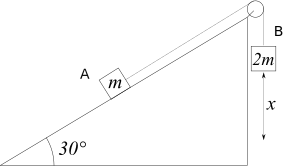
\includegraphics[width=0.3\textwidth]{../../../figures/Dynamics_masses_slope_30.svg}
	\caption{}\label{fig:Dynamics_masses_slope_30}
\end{figure}
\nl
What is the speed of the particles after this motion?
\begin{enumerate}
	\item \quantity{\sqrt{\frac{5}{3}gx}}{}
	\item \quantity{\sqrt{\left(\frac{4 + \sqrt{3}}{3}\right)gx}}{}
	\item \quantity{\sqrt{\left(\frac{4 - \sqrt{3}}{3}\right)gx}}{}
	\item \quantity{\sqrt{gx}}{} \answer
	\item \quantity{\sqrt{\frac{1}{2}gx}}{}
\end{enumerate}
}
{\stress{Created for the Rutherford School Physics Project by PS.}}
{The correct answer is (d). In this question, the gravitational potential energy lost by \valuedef{B}{2mgx}{}. The gravitational potential energy gained by \vari{A} $=$ \valuedef{mgx\sin{30^{\circ}}}{\frac{1}{2}mgx}{}, so the total GPE lost $=$ \valuedef{2mgx - \frac{1}{2}mgx}{\frac{3}{2}mgx}{}. This is equal to the total kinetic energy gained by both particles: \valuedef{\frac{1}{2}\left(3m\right)v^{2}}{\frac{3}{2}mgx}{}. Rearrange this equation to obtain the answer.
}
\end{problem}